\documentclass[reqno,a4paper,12pt]{amsart}

\usepackage{amsmath,amssymb,amsthm,geometry,xcolor,soul,graphicx}
\usepackage{mathrsfs} %\mathscr{}
%\usepackage{array}
\usepackage{float} % 在tcolorbox中添加table (由于tcolorbox已经是一个box,因此不能直接加table)
\usepackage{subfig} % 多张图放一起
\usepackage{titlesec}
%\usepackage{enumitem}
\usepackage{enumerate}
\usepackage{lipsum}
\usepackage{listings}
\allowdisplaybreaks[4] %align公式跨页
\RequirePackage[most]{tcolorbox}
\usepackage{braket}
%\usepackage{esint} %$\varoiint$ (带圈的二重积分)
%\usepackage[colorlinks,linkcolor=red]{hyperref} %\url{}超链接
\usepackage[scheme=plain,linespread=1,punct=CCT]{ctex}% Chinese support, single line space, narrow-version SBC case punctuations
\setCJKfamilyfont{zhsong}[AutoFakeBold={2.17}]{SimSong-Regular}
\renewcommand{\songti}{\CJKfamily{zhsong}}
%\usepackage{xeCJK}
%\setCJKmainfont{Kai}
\geometry{left=0.7in, right=0.7in, top=1in, bottom=1in}

\renewcommand{\baselinestretch}{1.3}

\title{固体物理第十三次作业}
\author{董建宇 ~~ 2019511017}

\begin{document}

\maketitle

\begin{enumerate}[1.]

\item \textbf{(19.4) $\ddagger$ Para and Diamagnetism} \\
Manganese (Mn, atomic number = 25) forms an atomic vapor at 2000K with vapor pressure $10^5$ Pa. You can consider this vapor to be ideal gas. \\
(a) Determine $L$, $S$, and $J$ for an isolated manganese atom. Determine the paramagnetic contribution to the (Curie) susceptibility of this gas at 2000K. \\
(b) In addition to the Curie susceptibility, the manganese atom will also have some diamagnetic susceptibility due to its filled core orbitals. Determine the Larmor diamagnetism of the gas at 2000K. You may assume the atomic radius of an Mn atom is one {\AA}ngstrom. Make sure you know the derivations of all the formulas you use!
\begin{tcolorbox}[breakable, colframe = black, colback = black!5!white]
\begin{enumerate}[(a)]
\item Mn原子核外电子排布为$[\text{Ne}]3s^23p^63d^54s^2$,则总轨道角动量为$L=0$,总自旋角动量为$S=5/2$,则自旋轨道耦合角动量为$J=5/2$。则Hamiltonian为:
\[
	\mathcal{H} = \mu_B\mathbf{B} \cdot (\mathbf{L}+g\mathbf{S}).
\]
由于轨道角动量和自旋角动量算符分别和总角动量算符对易,则有:
\[
	\mathbf{B} \cdot (\mathbf{L}+g\mathbf{S}) = \mathbf{B} \cdot \mathbf{J} \left( \frac{\mathbf{L} \cdot \mathbf{J}}{\vert \mathbf{J} \vert^2} + g\frac{\mathbf{S} \cdot \mathbf{J}}{\vert \mathbf{J} \vert^2} \right) = \tilde{g} \mathbf{B} \cdot \mathbf{J}.
\]
其中等效$g$因子为:
\[
	\tilde{g} = \frac{1}{2}(g+1) + \frac{1}{2}(g-1)\frac{S(S+1)-L(L+1)}{J(J+1)}.
\]
对于Mn原子,等效$g$因子为:$\tilde{g} = 2$。则配分函数为:
\[
	Z = \sum_{J_z=-J}^J e^{-\beta\tilde{g} \mu_BB J_z} = \frac{e^{5\beta\mu_BB}-e^{-7\beta\mu_BB}}{1-e^{-2\beta\mu_BB}}.
\]
则每个原子的磁矩为:
\[
	m = k_BT \frac{\partial \log Z}{\partial B} = \mu_B \frac{6\cosh(6\beta\mu_BB)\sinh(\beta\mu_BB)-\sinh(6\beta\mu_BB)\cosh(\beta\mu_BB)}{\sinh(\beta\mu_BB)\sinh(6\beta\mu_BB)}.
\]
则磁化率为:
\[
	\chi = \lim_{H\to 0} \frac{\partial nm}{\partial H} = \frac{35}{3}n\beta\mu_0\mu_B^2 = \frac{35}{3}\beta^2P\mu_0\mu_B^2.
\]
其中$n$为单位体积的原子数,$P$为压强。代入数据可得:
\[
	\chi = 1.65\times 10^{-7}.
\]

\item 假设磁场方向沿$z$方向,则反铁磁Hamiltonian的本征值为:
\[
	E_0 = \frac{e^2}{8m} \langle \vert \mathbf{B} \times \mathbf{r} \vert^2 \rangle = \frac{e^2B^2}{8m}\langle x^2 + y^2 \rangle.
\]
由于球对称性,可有:
\[
	\langle x^2+y^2 \rangle = \frac{2}{3}\langle r^2 \rangle.
\]
则单个原子磁矩为:
\[
	m_0 = -\frac{\partial E_0}{\partial B} = -\frac{e^2B}{6m}\langle r^2 \rangle.
\]
磁化率为:
\[
	\chi = \lim_{H\to 0} \frac{\partial (25nm)}{\partial H} = -\frac{25\mu_0e^2P\beta\langle r^2 \rangle}{6m} = -5.34\times 10^{-9}.
\]
\end{enumerate}
\end{tcolorbox}

\item \textbf{(19.6) $\ddagger$ Paramagnetism} \\
Consider a gas of monatomic atoms with spin $S = 1/2$ (and $L=0$) in a magnetic field $B$. The gas has density $n$. \\
(a) Calculate the magnetization as a function of $B$ and $T$. Determine the susceptibility. \\
(b) Calculate the contribution to the specific heat of this gas due to the spins. Sketch this contribution as a function of $\mu_BB/k_BT$.
\begin{tcolorbox}[breakable, colback = black!5!white, colframe = black]
\begin{enumerate}[(a)]

\item 对于自旋为$S = 1/2$,轨道角动量$L=0$的原子,自旋轨道耦合的角动量的取值为$J=1/2$。则有效$g$因子为
\[
	\tilde{g} = 2.
\]
则配分函数为:
\[
	Z = e^{-\beta\mu_BB} + e^{\beta\mu_BB}.
\]
则系统自由能为:
\[
	F = -kT\ln Z.
\]
单个原子的磁矩为:
\[
	m = -\frac{\partial F}{\partial B} = \mu_B \tanh(\beta\mu_BB).
\]
单位体积的磁矩为:
\[
	M = mn = n\mu_B\tanh(\beta\mu_BB).
\]
磁化率为:
\[
	\chi = \lim_{B\to0} \frac{\partial M }{\partial H} = n\mu_0 \beta\mu_B^2.
\]

\item 利用配分函数可以求内能为:
\[
	U = -\frac{\partial \ln Z}{\partial \beta} = -\mu_BB \tanh(\beta\mu_BB).
\]
热熔为:
\[
	C = \frac{\partial U}{\partial T} = \frac{(\mu_BB)^2}{kT^2} \frac{1}{\cosh^2(\beta\mu_BB)}.
\]
令$x = \mu_BB/kT = \beta\mu_BB$,热熔可以写为:
\[
	C = \frac{x^2}{k\cosh^2(x)}.
\]
绘图如下:
\begin{figure}[H]
	\centering
	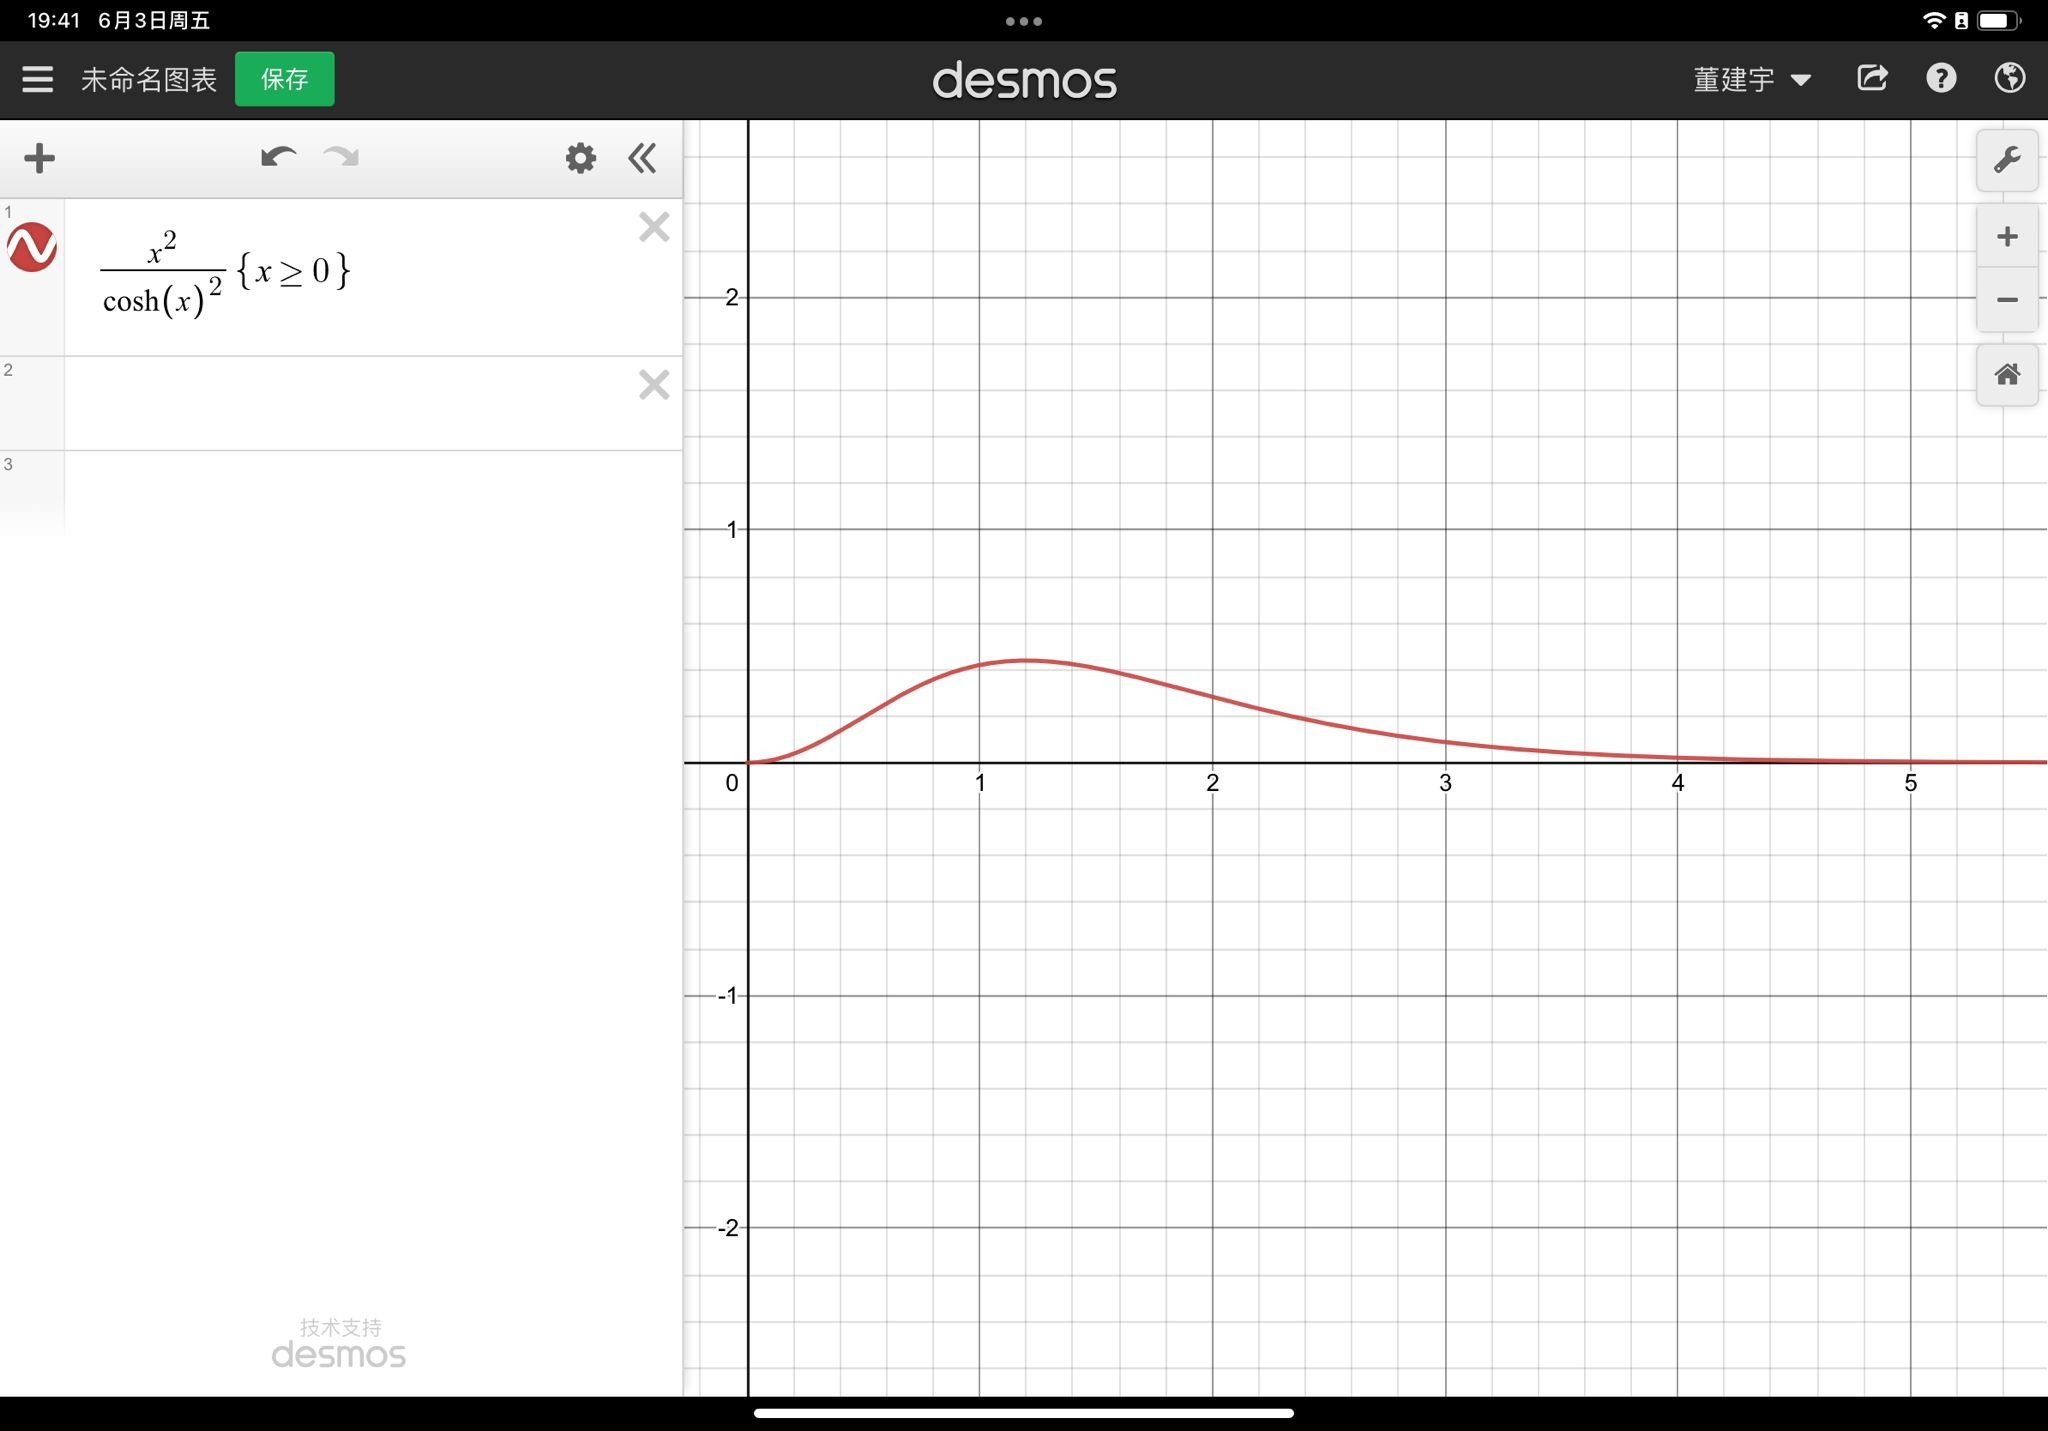
\includegraphics[width = 120mm]{19.6.jpg}
	\caption{热熔随$\mu_BB/kT$变化曲线}
\end{figure}


\end{enumerate}
\end{tcolorbox}

\item \textbf{(20.1) Ferromagnetic vs Antiferromagnetic States} \\
Consider the Heisenberg Hamiltonian 
\[
	\mathcal{H} = -\frac{1}{2} \sum_{<i,j>} J\mathbf{S}_i \cdot \mathbf{S}_j + \sum_i g\mu_B \mathbf{B} \cdot \mathbf{S}_i
\]
and for this exercise set $\mathbf{B} = 0$. \\
(a) For $J>0$, i.e., for the case of a ferromagnet, intuition tells us that the ground state of this Hamiltonian should simply have all spins aligned. Consider such a state. Show that this is an eigenstate of the Hamiltonian Eq. 20.6 and find its energy. \\
(b) For $J<0$, the case of an antiferromagnnet on a cubic lattice, one might expect that (at least for $\mathbf{B} = 0$) the state where spins on alternating sites point in opposite directions might be an eigenstate. Unfortunately, this is not precisely true. Consider such a state of the system. Show that the state in question is not an eigenstate of the Hamiltonian. \\
Although the intuition of alternating spins on alternating sites is not perfect, it becomes reasonable for systems with large spins $S$. For smaller spins (like spin $1/2$) one needs to consider so-called "quantum fluctuations" (which is much more advanced, so we will not do that here).
\begin{tcolorbox}[breakable, colframe = black, colback = black!5!white]
\begin{enumerate}[(a)]

\item 当$J>0$时,相邻自旋更趋向于平行方向,即形成铁磁态,态矢量为$\ket{\uparrow_i,\uparrow_j}$,则可以验证,在磁感应强度为$\mathbf{B} = 0$时,有:
\[
	\mathbf{S}_i \cdot \mathbf{S}_j \ket{\uparrow_i,\uparrow_j} = \left( \frac{1}{2}(S_+^iS_-^j + S_-^iS_+^j) + S_z^iS_z^j \right) \ket{\uparrow_i,\uparrow_j} = m_s^2 \ket{\uparrow_i,\uparrow_j}.
\]
即右矢$\ket{\uparrow_i,\uparrow_j}$为Hamiltonian的本征态,同理,两自旋都向下时也为Hamiltonian的本征态。此时,在选取磁感应强度为$\mathbf{B} = 0$时,总能量为:
\[
	E = \frac{1}{2}N\alpha JS^2.
\]
其中$N$为总自旋数目,$\alpha$为每个自旋近邻自旋数。

\item 考虑两个自旋反平行的态$\ket{\uparrow_i,\downarrow_j}$,则有:
\[
	\mathbf{S}_i \cdot \mathbf{S}_j \ket{\uparrow_i,\downarrow_j} = \left( \frac{1}{2}(S_+^iS_-^j + S_-^iS_+^j) + S_z^iS_z^j \right) \ket{\uparrow_i,\downarrow_j} = S^2(2\ket{\downarrow_i,\uparrow_j} + \ket{\uparrow_i,\downarrow_j}).
\]
即两个自旋反平行的态并不是Hamiltonian的本征态。

\end{enumerate}
\end{tcolorbox}

\item \textbf{(20.4) Small Heisenberg Models} \\
(a) Consider a Heisenberg model containing a chain of only two spins, so that 
\[
	\mathcal{H} = -J\mathbf{S_1}\cdot\mathbf{S_2}.
\]
Supposing these spins have $S=1/2$, calculate the energy spectrum of this system. Hint: Write $2\mathbf{S_1\cdot S_2} = (\mathbf{S_1} + \mathbf{S_2})^2 - \mathbf{S_1}^2 - \mathbf{S_2}^2$. \\
(b) Now consider three spins forming a triangle (as shown in Fig. 20.2). Again assuming these spins are $S = 1/2$, calculate the spectrum of the system. Hint: Use the same trick as in part (a)! \\
(c) Now consider four spins forming a tetrahedron. Again assuming these spins are $S = 1/2$, calculate the spectrum of the system.
\begin{tcolorbox}[breakable, colframe = black, colback = black!5!white]
\begin{enumerate}[(a)]

\item 可以令$\mathbf{J_1} = \mathbf{S_1}+\mathbf{S_2}$,由于自旋均为$S=1/2$,则$J_1$的可能取值为:$1$或$0$,则能量分别为:
\begin{align*}
	E_{J_1=1} =& -J\times \frac{1\times 2 - \frac{1}{2}\times\frac{3}{2} - \frac{1}{2}\times\frac{3}{2}}{2} = -\frac{J}{4}; \\
	E_{J_1=0} =& -J\times \frac{0 - \frac{1}{2}\times\frac{3}{2} - \frac{1}{2}\times\frac{3}{2}}{2} = \frac{3}{4}J.
\end{align*}
简并度分别为:
\[
	g_{J_1 = 1} = 3, ~ g_{J_1=0} = 1.
\]

\item 当有三个自旋组成三角形状时,Hamiltonian写为:
\[
	\mathcal{H} = -J(\mathbf{S_1\cdot S_2} + \mathbf{S_1\cdot S_3} + \mathbf{S_2\cdot S_3}) = -\frac{J}{2}((\mathbf{S_1} + \mathbf{S_2} + \mathbf{S_3})^2 - \mathbf{S_1}^2 - \mathbf{S_2}^2 - \mathbf{S_3}^2).
\]
令$\mathbf{J_2} = \mathbf{S_1} + \mathbf{S_2} + \mathbf{S_3}$,则$J_2$的可能取值为:$\frac{1}{2}$或$\frac{3}{2}$,则能量分别为:
\begin{align*}
	E_{J_2 = 1/2} =& \frac{3J}{4}; \\
	E_{J_2 = 3/2} =& -\frac{3J}{4}
\end{align*}
简并度分别:
\[
	g_{J_2 = 1/2} = 4, ~ g_{J_2=3/2} = 4.
\]

\item 当有四个自旋时,Hamiltonian可以写为:
\[
	\mathcal{H} = -\frac{J}{2}((\mathbf{S_1} + \mathbf{S_2} + \mathbf{S_3} + \mathbf{S_4})^2 - \mathbf{S_1}^2 - \mathbf{S_2}^2 - \mathbf{S_3}^2 - \mathbf{S_4}^2).
\]
令$\mathbf{J_3} = \mathbf{S_1} + \mathbf{S_2} + \mathbf{S_3} + \mathbf{S_4}$,则$J_3$的可能取值为:$0,1,2$,能量分别为:
\begin{align*}
	E_{J_3 = 0} =& \frac{3J}{2}; \\
	E_{J_3 = 1} =& \frac{J}{2}; \\
	E_{J_3 = 2} =& -\frac{3J}{2}.
\end{align*}
简并度分别:
\[
	g_{J_3 = 0} = 2, ~ g_{J_3=1} = 9, ~ g_{J_3 = 2} = 5.
\]

\end{enumerate}
\end{tcolorbox}

\item \textbf{(20.5) One-Dimensional Ising Model with $B=0$} \\
(a) Consider the one-dimensional Ising model with spin $S=1$. We write the Hamiltonian for a chain of $N$ spins in zero magnetic field as 
\[
	\mathcal{H} = -J\sum_{i=1}^{N-1} \sigma_i\sigma_{i+1}
\]
where each $\sigma_i$ takes the value $\pm1$. The partition function can be written as 
\[
	Z = \sum_{\sigma_1,\sigma_2,\cdots,\sigma_N} e^{-\beta H}.
\]
Using the transformation $R_i = \sigma_i\sigma_{i+1}$ rewrite the partition function as a sum over the $R$ variables, and hence evaluate the partition function. \\
$\triangleright$ Show that the free energy has no cusp or discontinuity at any temperature, and hence conclude that there is no phase transition in the one-dimensional Ising model. \\
(b)${ }^*$ At a given temperature $T$, calculate an expression for the probability that $M$ consecutive spins will be pointing in the same direction. How does this probability decay with $M$ for large $M$? What happens as $T$ becomes small? You may assume $N\gg M$.
\begin{tcolorbox}[breakable, colframe = black, colback = black!5!white]
\begin{enumerate}[(a)]

\item 令$R_i = \sigma_i \sigma_{i+1}$,Hamiltonian可以写为:
\[
	\mathcal{H} = -J\sum_{i=1}^{N-1} R_i.
\]
则配分函数为:
\[
	Z = \sum_{\sigma_1,\sigma_2,\cdots,\sigma_N} \prod_{i=1}^{N-1} e^{-\beta JR_i} = 2\prod_{i=1}^{N-1} \sum_{R_i=\pm1} e^{-\beta JR_i} = 2(e^{\beta J} + e^{-\beta J})^{N-1}.
\]
$\triangleright$ 则自由能为:
\[
	F = -k_BT \ln Z = k_BT\ln2 - k_BT(N-1)\ln(e^{\beta J} + e^{-\beta J}).
\]
自由能对温度的导数为:
\[
	\frac{\partial F}{\partial T} = -k_B(N-1)\ln(e^{\beta J} + e^{-\beta J}) + \frac{(N-1)J}{T}\tanh(\beta J).
\]
即自由能关于温度是一个连续函数,不存在尖峰,也就意味着一维Ising模型没有相变。

\item 考虑题目意思理解为存在$M$个相邻的自旋朝向相同,注意到当$R_i = \sigma_i\sigma_{i+1} = 1$就意味着两自旋平行,若$R_i=-1$,则两自旋反平行,可以计算,$R_i = 1$的概率为:
\[
	P(R_i = 1) = \frac{e^{\beta J}}{e^{\beta J} + e^{-\beta J}}.
\]
则存在$M$个平行自旋相邻的概率为:
\[
	P_0 = (P(R_i=1))^{M-1} = (1+e^{-2\beta J})^{1-M}.
\]
研究概率随$M$的变化时,可以改写得:
\[
	P_0 = \exp((1-M)\ln(1+e^{-2\beta J})).
\]
即在给定的温度下,概率随$M$的增加指数减小。 \\
当温度$T$减小时,$\beta = 1/k_BT$增加,则概率$P_0$减小,当温度趋向于$0K$时,概率趋向于$P_0 = 1$,即所有粒子自旋平行。
\end{enumerate}
\end{tcolorbox}

\item \textbf{补充题}: 推导并画出外磁场沿一个 single magnetic domain 的hard axis 时,其磁滞回线。请注意,如下图数据所示,对于理想的single domain,沿着easy axis的磁滞回线是一个矩形,而沿着hard axis是一条直线。
\begin{tcolorbox}[breakable, colframe = black, colback = black!5!white]
Hamiltonian可以写为:
\[
	\mathscr{H} = -\frac{1}{2}J\sum_{<i,j>} \vec{S}_i\cdot\vec{S}_j - \kappa \sum_i {S_i^z}^2.
\]
则考虑单畴,当施加外磁场沿x轴(即hard axis),能量可以写为:
\[
	E = -BM\sin\alpha\sin\theta - \kappa M^2\cos^2\theta = \kappa M^2 \sin^2\theta - BM\sin\alpha\sin\theta - \kappa M^2.
\]
其中$\theta$为磁化强度与z轴夹角,$\alpha$为磁化强度在$xy$平面内的投影与$x$轴方向夹角。绘制能量随$\sin\theta$的函数图像,可以注意到,当$0 \leq \frac{B\sin\alpha}{2\kappa M} \leq 1$时,能量最小值对应$\sin\theta = \frac{B\sin\alpha}{2\kappa M}$,此时能量为:
\[
	E_1 = -\frac{B^2\sin^2\alpha}{4\kappa} - \kappa M^2.
\]
所以有能量最小值时磁化强度与外加磁场的磁感应强度满足:
\[
	M = \frac{\sin\alpha}{2\kappa\sin\theta}B.
\]
当$\frac{B\sin\alpha}{2\kappa M} > 1$时,能量最小值对应$\sin\theta=1$,此时磁化强度将不再变化。 \\
当$\frac{B\sin\alpha}{2\kappa M}$不同取值时的能量随$\sin\theta$变化曲线:
\begin{figure}[H]
	\centering
	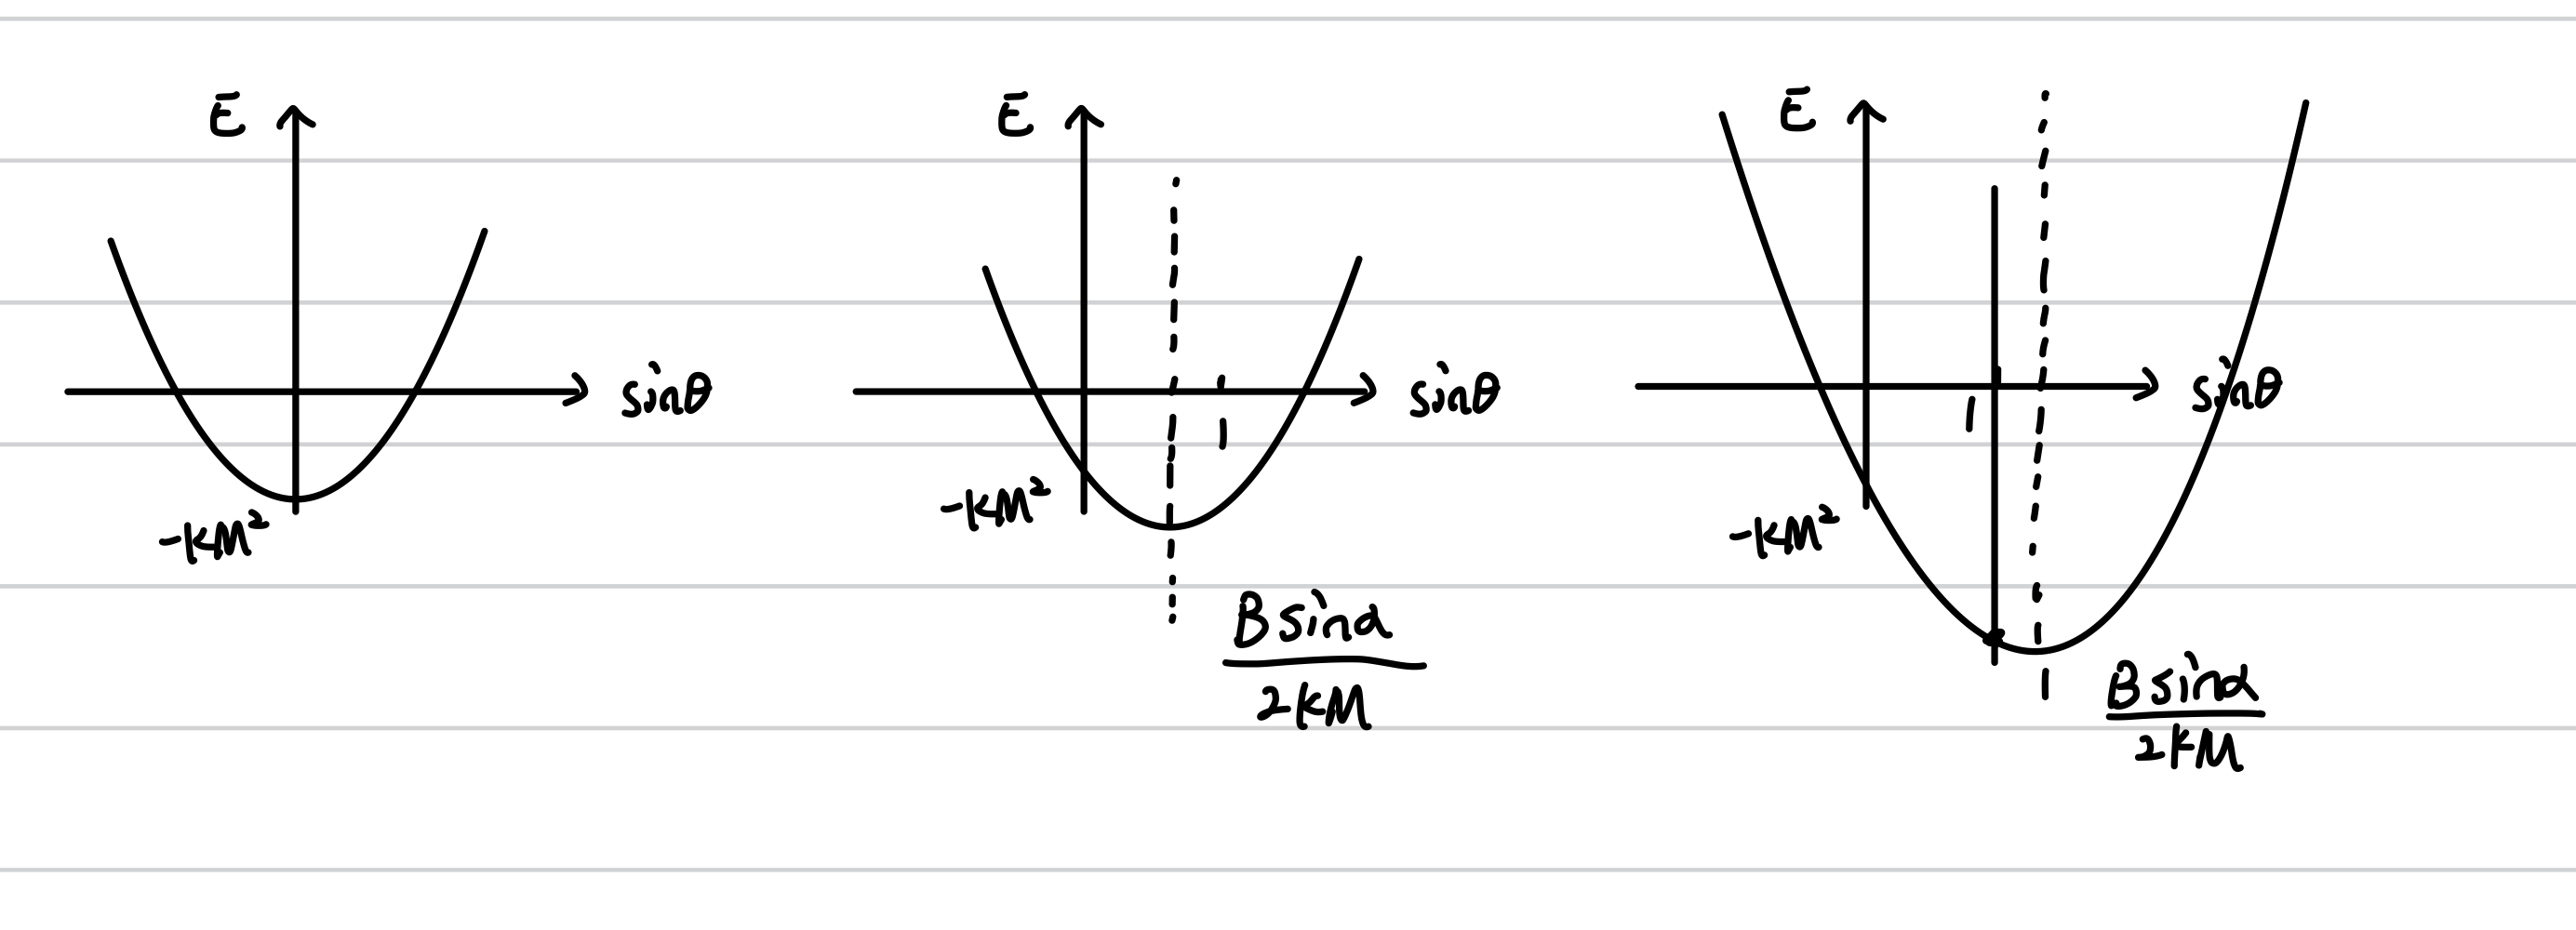
\includegraphics[width = 120mm]{sintheta.jpeg}
	\caption{\text{$\frac{B\sin\alpha}{2\kappa M}$不同取值时的能量随$\sin\theta$的变化曲线}}
\end{figure}
同理可知,当$\frac{B\sin\alpha}{2\kappa M}<0$时的情况,则可以画出磁化强度随外加磁场变化曲线:
\begin{figure}[H]
	\centering
	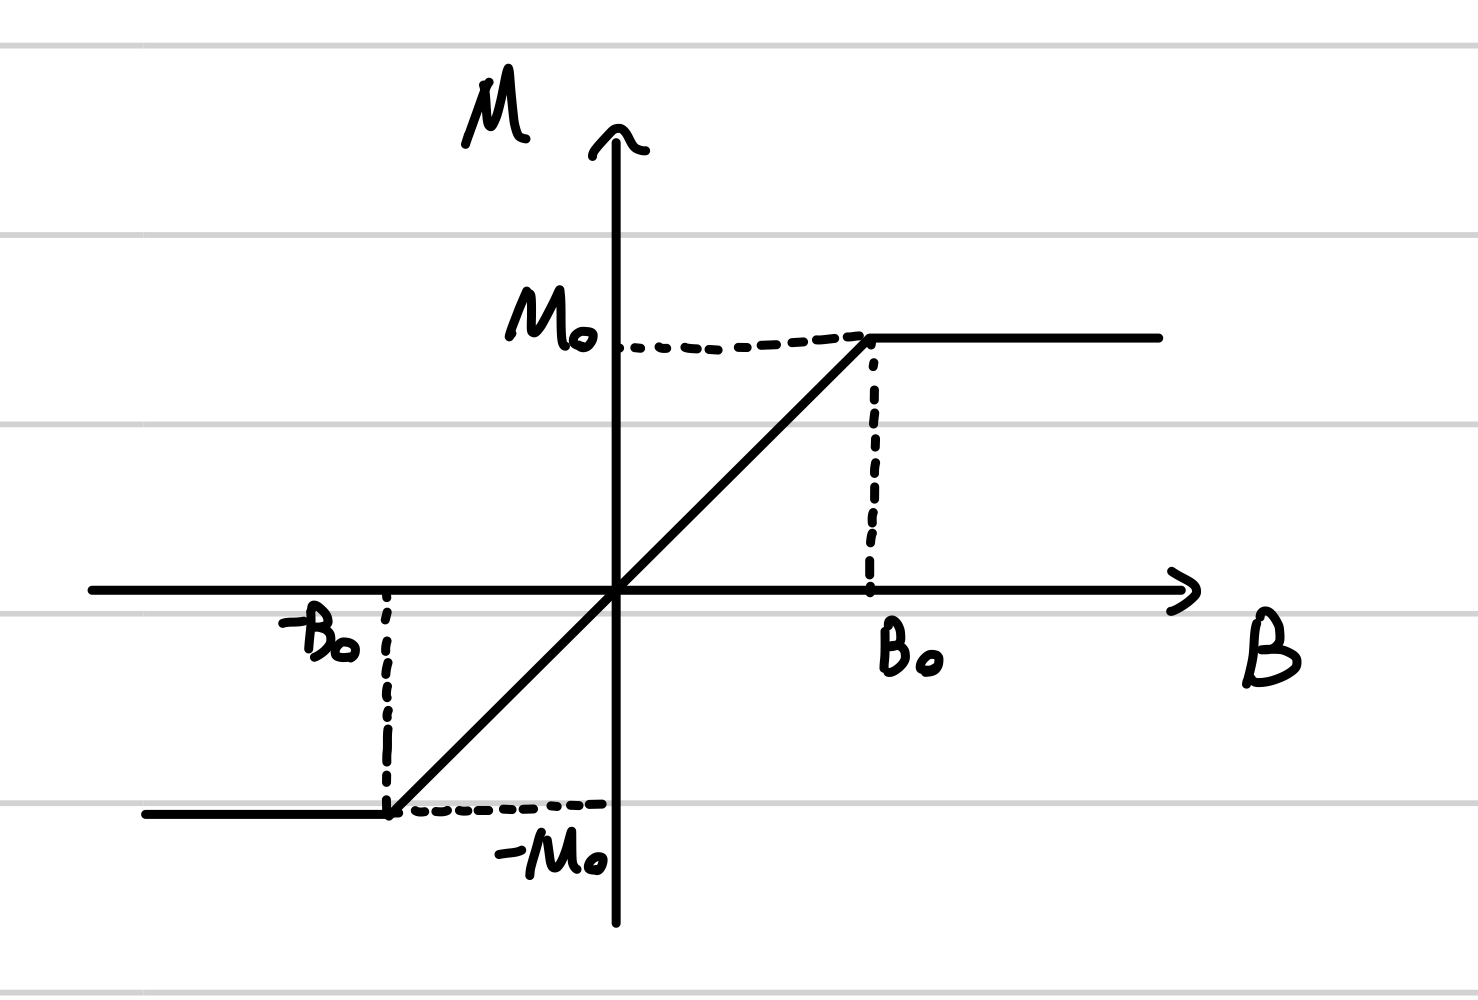
\includegraphics[width = 120mm]{M-B.jpeg}
	\caption{\text{磁化强度随磁感应强度变化曲线}}
\end{figure}


\end{tcolorbox}

\end{enumerate}

\end{document}